%-----------------------------
%-----------------------------
\chapter{Zusätzliche Features}
\label{chapter:additional_features}


%---------------------------
\section{Benutzeroberfläche}
\label{gui}

Mit dem in Kapitel \ref{chapter:skeleton_generation} vorgestellen Algorithmus können nicht nur zufällige Skelette generiert werden. Über eine Benutzeroberfläche ist es auch möglich dem Algorithmus zusätzliche Eingaben zu geben. Die Benutzeroberfläche ist in Abbildung \ref{gui_screenshot} zu sehen.
Im Folgenden ist für alle möglichen Eingaben beschrieben, wie sie in Bedingungen für die PCA umgesetzt werden. Ist in Zahlenfeldern nichts eingegeben, haben diese keinen Einfluss auf den Ablauf (im Gegensatz zur Eingabe der Zahl $0$).

\begin{figure}[ht]
 \centering
 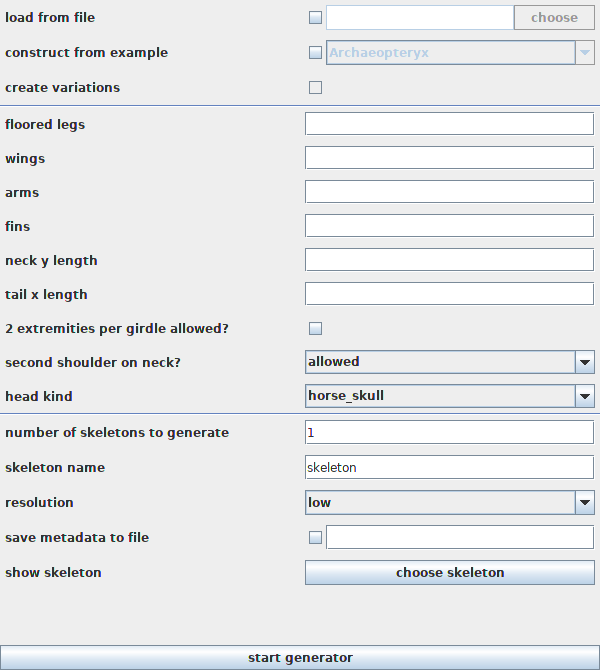
\includegraphics[width=0.7\textwidth]{graphics/gui.png}
 \caption{Die Benutzeroberfläche des Programms. Der Knopf "`start generator"' startet den Algorithmus mit den zusätzlichen Eingaben aus den Feldern darüber.}
 \label{gui_screenshot}
\end{figure}

\begin{itemize}
 \item Die Anzahl der Beine (floored legs) mit Bodenkontakt muss eine gerade Zahl $n$ zwischen $0$ und $8$ sein. Die Hälfte wird als Bedingung für \emph{Paare von Beinen mit Bodenkontakt} an die PCA weitergegeben, wie in Abschnitt \ref{pca_conditions} beschrieben. Bei echten Wirbeltieren liegt diese Anzahl zwischen $0$ und $4$. Werden Werte größer $4$ als Bedingung an die PCA gestellt, so werden sehr stark geschwungene Wirbelsäulen generiert. Diese sehen aber, bis zu einem Wert von ca.\ $8$ nicht schlecht aus. Deshalb werden diese Werte auch als Bedingungen erlaubt. Sie werden nur mit einer gewissen Wahrscheinlichkeit etwas verkleinert, weil fantastische Tiere mit mehr als $4$ Beinen auch mit Wirbelsäulen für Tiere mit $4$ Beinen generiert werden können.
 
 \item Die Anzahl der Flügel (wings) muss ebenfalls gerade sein. Die Hälfte des Eingabewerts, aber maximal $1$, wird als Bedingung an die PCA weitergegeben.
 Im Gegensatz zu den Beinen sind die Wirbelsäulen, die unter Bedingungen größer $1$ für \emph{Flügel} generiert werden, mit großer Wahrscheinlichkeit unrealistisch.
 
 \item Die Zahlen für Arme (arms) und Flossen (fins) gehen nicht als Bedingung in die PCA ein.
 
 \item Die $y$-Komponente des Abstands zwischen Kopf und Schultergürtel (neck $y$ length) und die $x$-Komponente des Abstands zwischen Hüfte und Schwanzspitze (tail $x$ length) können wiederum direkt als Bedingung an die PCA weitergegeben werden. Auch hier werden, wie auch bei Beinen und Flügeln (wie in Abschnitt \ref{pca_conditions} beschrieben), zufällige kleine Werte aufaddiert oder abgezogen um mehr Variation auf den erzeugten Skeletten zu bekommen.
\end{itemize}

Die Anzahlen der verschiedenen Extremitätentypen werden außerdem verwendet um die Parameter $e_v, e_h$ und $e_v2$ für die Anzahl der Vorder- und Hinterextremitäten der Grammatik (siehe Abschnitte \ref{section:grammar} und \ref{additional_extremities}) zu bestimmen und um den Typ und damit die Positionierung der verschiedenen generierten Extremitäten festzulegen (siehe Anfang \mbox{Abschnitt \ref{section:extremity_generation}}). Zusätzlich muss mit einberechnet werden ob zwei Extremitätenpaare pro Extremitätengürtel erlaubt sind ($2$ extremities per girdle allowed?) und ob ein zweiter Schultergürtel auf dem Hals erlaubt, erzwungen oder verboten ist (second shoulder on neck?) (siehe auch Abschnitt \ref{additional_extremities}).

Außerdem gibt es theoretisch noch die Möglichkeit anzugeben welches 3D-Modell für den Kopf verwendet werden soll (head kind). Leider gibt es hier, Stand Abschluss der Arbeit, nur eines zu Auswahl. Dies ließe sich aber leicht anpassen (siehe Abschnitt \ref{bone_models}).
Zusätzlich kann eingestellt werden welche Auflösung das 3D-Modell haben soll (resolution). Hier gibt es die Möglichkeit nur Quader zu generieren oder Modelle von echten Knochen in niedriger oder hoher Auflösung einzusetzen.

Im Feld "`skeleton name"' kann eingestellt werden wieviele Skelette auf einmal generiert werden sollen. Und schließlich kann man sich auch ein generiertes Modell anzeigen lassen (show skeleton). Dazu wird das Programm \emph{JavaView} \cite{JavaView} verwendet. Es ist darauf spezialisiert 3D-Geometrie interaktiv zu visualisieren und kann in Javacode eingebunden werden.


%------------------------------------------
\section{Speichern und Laden von Skeletten}
\label{load_skeletons}

Um ein vorgegebenes Skelett reproduzieren zu können reicht es einige Metadaten zu speichern. Dazu gehören die Dimensionen der PCA (Position der Wirbelsäule, Länge der Knochen in den Extremitäten und Gewicht) und Daten, die zusätzlich generiert werden (Anzahl und Art der Extremitäten an den jeweiligen Extremitätengürteln, die Winkel an den Gelenken der Extremitäten, Anzahl der Wirbel und Rippen und welches 3D-Modell für den Kopf verwendet werden soll).
Das alles wird in wenigen Java-Klassen gebündelt. So können die Daten über Java-Serialisierung \cite{JavaSerialization} in eine Textdatei geschrieben. Diese Datei kann dann wieder eingelesen werden um die Klassen wieder herzustellen.

Im Benutzerinterface (Abbildung \ref{gui_screenshot}) kann diese Funktion verwendet werden, indem "`save metadata to file"' ausgewählt wird und ein Dateiname eingegeben wird. Dann wird für jedes generierte Skelett eine Textdatei mit dem angegebenen Namen generiert, die die serialisierten Daten enthält.\\
Um ein Skelett aus solch einer Textdatei zu laden, muss die entsprechende Datei bei "`load from file"' ausgewählt werden. Dann werden die dazugehörigen Java-Klassen wieder hergestellt und das gleiche 3D-Modell noch einmal generiert.

Das funktioniert natürlich nur über das implementierte Programm, das genau die serialisierten Java-Klassen enthält und liefert keine Zusatzinformationen zu dem generierten Skelett an den Benutzer. Solche Zusatzinformationen könnten in weiterführenden Arbeiten generiert werden. Hilfreiche Informationen könnten \zb die Knochenhierarchie oder die Winkeleinschränkungen an den Gelenken sein.

Zusätzlich gibt es die Funktion konkrete PCA-Eingabebeispiele auszuwählen (construct from example). Dann wird ein Skelett mit den Daten generiert, die für dieses Beispiel erhoben wurden. Mit einem PCA-Punkt sind aber noch nicht alle Daten festgelegt, die ein Skelett bestimmen. Es ist nur festgelegt welcher PCA-Punkt in Schritt 2 des Algorithmus ausgewählt wird, nicht welche konkreten Parameter die Grammatik bekommt oder welche Typen von Extremitäten generiert werden (siehe Abschnitt \ref{section:overview}). Deshalb ist es zusätzlich möglich weitere Bedingungen \zb für die Anzahl der Arme einzugeben.


%---------------------------------
\section{Erzeugung von Variationen}

\begin{itemize}
 \item was genau wird variiert
 \item kann verwendet werden um schnell verschiedene Möglichkeiten zu testen
 \item PCA Daten normalverteilt variieren (Verteilung bleibt Gauß, Erwartungswert bleibt gleich, Überlegungen dazu wie sie sich ändert durch Aufaddieren der Variation / Faltung mit anderem Gauß)
 \item Variation der Daten, die nicht von PCA abhängen, beschreiben; generische Algorithmen zitieren (auch hinzufügen und löschen oder ändern von Features um Variationen/Verbesserungen zu erzeugen)
 \item create variations on existing models: simmons wilhelms van gelder 2002
	\url{https://www.researchgate.net/publication/234776823_Model-based_reconstruction_for_creature_animation}
\end{itemize}

